\documentclass[letterpaper]{article}
\usepackage[margin=1in]{geometry}
\usepackage[utf8]{inputenc}
\usepackage{textcomp}
\usepackage{amssymb}
\usepackage{natbib}
\usepackage{graphicx}
\usepackage{gensymb}
\usepackage{amsthm, amsmath, mathtools}
\usepackage[dvipsnames]{xcolor}
\usepackage{enumerate}
\usepackage{mdframed}
\usepackage[most]{tcolorbox}
\usepackage{csquotes}
% https://tex.stackexchange.com/questions/13506/how-to-continue-the-framed-text-box-on-multiple-pages

\tcbuselibrary{theorems}

\newcommand{\R}{\mathbb{R}}
\newcommand{\Z}{\mathbb{Z}}
\newcommand{\N}{\mathbb{N}}
\newcommand{\Q}{\mathbb{Q}}
\newcommand{\C}{\mathbb{C}}
\newcommand{\code}[1]{\texttt{#1}}
\newcommand{\mdiamond}{$\diamondsuit$}
\newcommand{\PowerSet}{\mathcal{P}}
\newcommand{\Mod}[1]{\ (\mathrm{mod}\ #1)}
\DeclareMathOperator{\lcm}{lcm}

%\newtheorem*{theorem}{Theorem}
%\newtheorem*{definition}{Definition}
%\newtheorem*{corollary}{Corollary}
%\newtheorem*{lemma}{Lemma}
\newtheorem*{proposition}{Proposition}


\newtcbtheorem[number within=section]{theorem}{Theorem}
{colback=green!5,colframe=green!35!black,fonttitle=\bfseries}{th}

\newtcbtheorem[number within=section]{definition}{Definition}
{colback=blue!5,colframe=blue!35!black,fonttitle=\bfseries}{def}

\newtcbtheorem[number within=section]{corollary}{Corollary}
{colback=yellow!5,colframe=yellow!35!black,fonttitle=\bfseries}{cor}

\newtcbtheorem[number within=section]{lemma}{Lemma}
{colback=red!5,colframe=red!35!black,fonttitle=\bfseries}{lem}

\newtcbtheorem[number within=section]{example}{Example}
{colback=white!5,colframe=white!35!black,fonttitle=\bfseries}{def}

\newtcbtheorem[number within=section]{note}{Important Note}{
        enhanced,
        sharp corners,
        attach boxed title to top left={
            xshift=-1mm,
            yshift=-5mm,
            yshifttext=-1mm
        },
        top=1.5em,
        colback=white,
        colframe=black,
        fonttitle=\bfseries,
        boxed title style={
            sharp corners,
            size=small,
            colback=red!75!black,
            colframe=red!75!black,
        } 
    }{impnote}
\usepackage[utf8]{inputenc}
\usepackage[english]{babel}
\usepackage{fancyhdr}
\usepackage[hidelinks]{hyperref}

\pagestyle{fancy}
\fancyhf{}
\rhead{MATH 155A}
\chead{Tuesday, March 29, 2022}
\lhead{Lecture 1}
\rfoot{\thepage}

\setlength{\parindent}{0pt}

\begin{document}

\section{Three Paradigms for Rendering}
We first begin by discussing how to render points, lines, and triangles. 

\subsection{Drawing Points}
Consider the following graph:
\begin{center}
    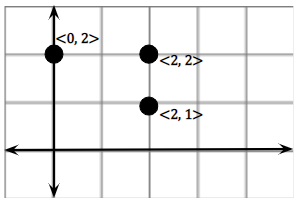
\includegraphics[scale=1]{../assets/points1.png}
\end{center}
In this class, we represent points in the form $\cyclic{x, y}$, or $\begin{bmatrix}
    x \\ y
\end{bmatrix}$. In C++, we can represent these points like so: 
\begin{verbatim}
    float verts[][2] = {
        {2, 1},
        {2, 2},
        {0, 2}
    };\end{verbatim}
After loading the array into the GPU, which we'll discuss later, we can use a command like: 
\begin{verbatim}
    glDrawArrays(GL_POINTS, 0, 3);\end{verbatim}

\subsection{Drawing Lines}
Consider the following graph:
\begin{center}
    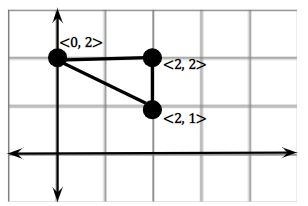
\includegraphics[scale=1]{../assets/line1.png}
\end{center}
In JavaScript, we can make use of the Canvas API to draw this like so: 
\begin{verbatim}
    moveTo(2, 1);
    lineTo(2, 2);
    lineTo(0, 2);
    lineTo(2, 2);
    stroke();\end{verbatim}
In OpenGL, we would do something like: 
\begin{verbatim}
    glDrawArrays(GL_LINE_LOOP, 0, 3);\end{verbatim}
The \code{GL\_LINE\_LOOP} means that we're making a closed loop of edges, using 3 vertices in total. 

\bigskip 

There are several other modes that we can use. To see how these differ, we'll use the following set of vertices as an example:
\begin{center}
    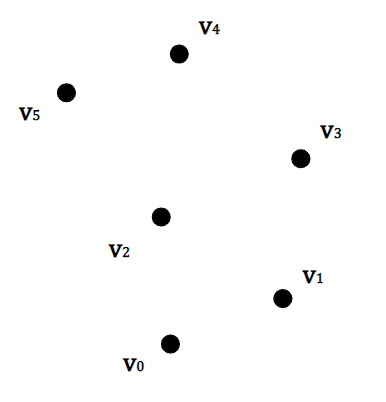
\includegraphics[scale=0.5]{../assets/points2.png}
\end{center}
\begin{itemize}
    \item \code{GL\_LINES}: If we have the following code segment
    \begin{verbatim}
        glDrawArrays(GL_LINES, 0, 6);\end{verbatim}
    Then, we would get the following drawing:
    \begin{center}
        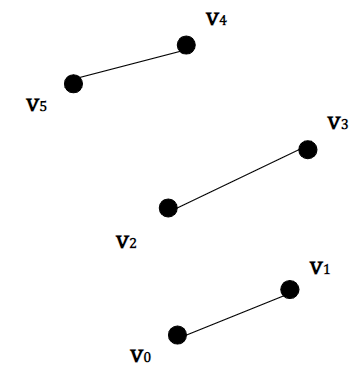
\includegraphics[scale=0.5]{../assets/points3.png}
    \end{center}

    \item \code{GL\_LINE\_STRIP}: Now, if we were to include the following code segment in addition to the one above
    \begin{verbatim}
        glDrawArrays(GL_LINES_STRIP, 0, 6);\end{verbatim}
    Then, we would get the following drawing: 
    \begin{center}
        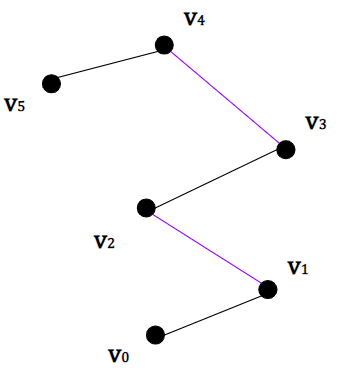
\includegraphics[scale=0.5]{../assets/points4.png}
    \end{center}

    \item \code{GL\_LINE\_LOOP}: Finally, including 
    \begin{verbatim}
        glDrawArrays(GL_LINES_LOOP, 0, 6);\end{verbatim}
    would yield the following drawing: 
    \begin{center}
        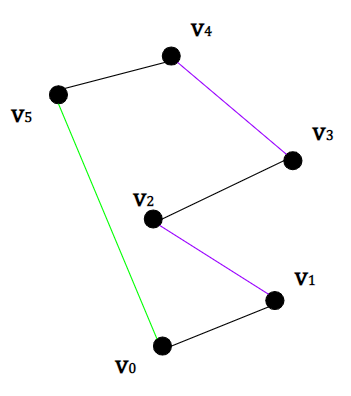
\includegraphics[scale=0.5]{../assets/points5.png}
    \end{center}
\end{itemize}


So, to sumamrize, if we have the vertices $\{v_1, v_2, \dots, v_n\}$, then: 
\begin{itemize}
    \item \code{GL\_LINES} will draw a line for each pair of vertices; that is, a line will be drawn between $v_1$ and $v_2$, $v_3$ and $v_4$, and so on. 
    \item \code{GL\_LINE\_STRIP} will draw a line for each consecutive pair of vertices, up to and including $v_{n - 1}$; that is, a line will be drawn between $v_1$ and $v_2$, $v_2$ and $v_3$, $v_3$ and $v_4$, and so on. The last line drawn will be from $v_{n - 1}$ to $v_{n}$. 
    \item \code{GL\_LINE\_LOOP} will draw a line for each consecutive pair of vertices, including from the end vertex to the start vertex. So, effectively, this is just \code{GL\_LINE\_STRIP} but with a line from $v_n$ to $v_1$.  
\end{itemize}

\subsection{Drawing Triangles}
Like with drawing lines, there are three modes for drawing triangles. 
\begin{itemize}
    \item \code{GL\_TRIANGLES}
    \item \code{GL\_TRIANGLE\_FAN}
    \item \code{GL\_TRIANGLE\_STRIP}
\end{itemize}
Using the same set of 6 points above, we show the following examples. 

\subsubsection{\code{GL\_TRIANGLES} Mode}
This mode groups the vertices into groups of three, and then draws a triangle between each group. For example, if you have vertices $\{v_0, \dots, v_5\}$, then this mode would take vertices $\{v_0, \dots, v_2\}$ and $\{v_3, \dots, v_5\}$ and draw a triangle (from $v_0 \to v_1$ and then from $v_1 \to v_2$ and finally $v_2 \to v_0$, while filling it in with a color).

\bigskip 

When we use the \code{GL\_TRIANGLES} mode, like so: 
\begin{verbatim}
    glDrawArrays(GL_TRIANGLES, 0, 6);
\end{verbatim}
Then we get something like: 
\begin{center}
    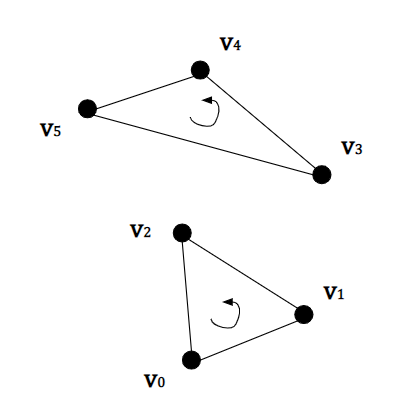
\includegraphics[scale=0.5]{../assets/triangle1.png}
\end{center}
Note that the arrows here indicate that we're looking at the ``front'' faces of the triangle. The ``back'' face is the other side. 

\subsubsection{\code{GL\_TRIANGLE\_FAN} Mode}
For an array of vertices $\{v_0, \dots, v_n\}$, $v_0$ is the common vertex. Then, the rest of the vertices $v_1, \dots, v_n$ are defining a triangle which shares the initial vertex.

\bigskip

Suppose you're given the following set of vertices like so: 
\begin{center}
    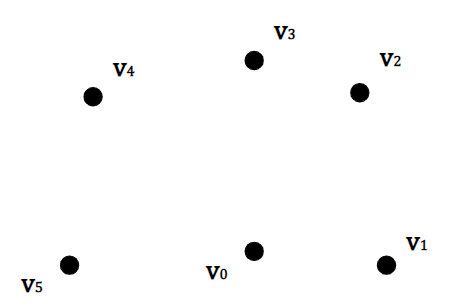
\includegraphics[scale=0.5]{../assets/triangle2.png}
\end{center}

When using this mode, like so 
\begin{verbatim}
    glDrawArrays(GL_TRIANGLE_FAN, 0, 6);
\end{verbatim}
Then we get something like: 
\begin{center}
    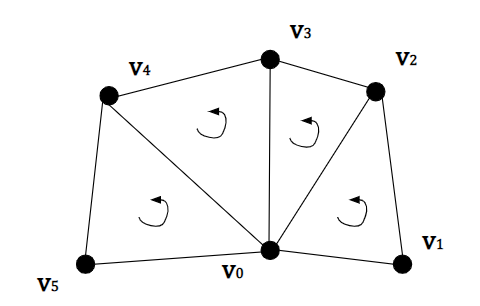
\includegraphics[scale=0.5]{../assets/triangle3.png}
\end{center}

\subsubsection{\code{GL\_TRIANGLE\_STRIP} Mode}
Suppose you're given the following set of vertices like so: 
\begin{center}
    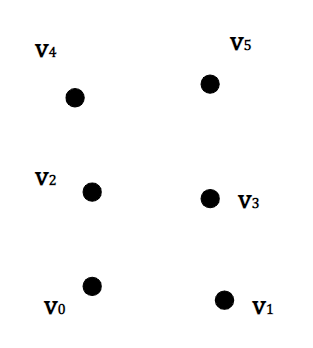
\includegraphics[scale=0.5]{../assets/triangle4.png}
\end{center}

When using this mode, like so 
\begin{verbatim}
    glDrawArrays(GL_TRIANGLE_STRIP, 0, 6);
\end{verbatim}
Then we get something like: 
\begin{center}
    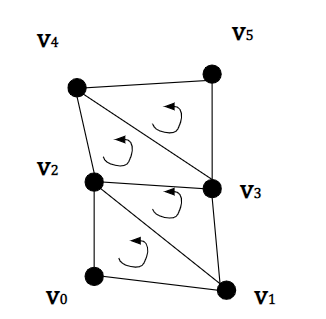
\includegraphics[scale=0.5]{../assets/triangle5.png}
\end{center}

The way to think about this is that you have your ``base'' triangle with vertices $\{v_0, v_1, v_2\}$. Then, $v_3$ is facing the edge formed between $v_1$ and $v_2$. Likewise, the vertex $v_4$ is facing the edge formed between $v_2$ and $v_3$ of the triangle with vertices $\{v_1, v_2, v_3\}$. 






\section{Culling, Hidden Surfaces, Animation}
Suppose you have a 3D scene, typically rendered as triangles. These will also typically be rendered with a view, i.e. camera, which has a position and direction.

\subsection{Culling}
Note that a triangle could be \emph{behind} the viewer. Or, maybe, the triangle is \emph{inside} the sphere. This gives us a definition. 
\begin{definition}{Cull}{}
    Meaning the same thing as discard, a \textbf{cull} is simply the triangles that are not visible to the viewer. 
\end{definition}
When rendering closed, solid, objects' surfaces, we can also cull back faces. 

\bigskip 

We can use the following OpenGL commands to enable cull back faces:
\begin{verbatim}
    glEnable(GL_CULL_FACE);\end{verbatim}
We can also specify which faces are culled. By default, the faces that are culled are the back faces. That is, the following is the default setting: 
\begin{verbatim}
    glCullFace(GL_BACK); // Default\end{verbatim}
We can also use the following commands: 
\begin{verbatim}
    glCullFace(GL_FRONT); // Cull front faces. 
    glCullFace(GL_FRONT_AND_BACK); // Cull all faces. \end{verbatim}
To disable culling, we can use: 
\begin{verbatim}
    glDisable(GL_CULL_FACE);\end{verbatim}
We can also change the conventions on counter-clockwise vs. clockwise, like so: 
\begin{verbatim}
    glFrontFace(GL_CCW); // Default \end{verbatim}
We can change this convention to make the opposite face the front face; that is, by using the following command: 
\begin{verbatim}
    glFrontFace(GL_CW);\end{verbatim}
Note that:
\begin{itemize}
    \item \code{CCW} means counter-clockwise.
    \item \code{CW} means clockwise.
\end{itemize}

\subsection{Hidden Surfaces Methods}
Here, the idea is that if there are some triangles that are in front of the other triangles, the other triangles are hidden. There are three methods for this. 
\begin{enumerate}
    \item \underline{Geometric Analysis:} Consider all pairs of triangles in the scene, figure out how they overlap with each other, and then render only the visible parts.  
    
    \bigskip 

    For example, suppose we have a green and red triangle, where the red triangle is partially in front of the green triangle. We would get something like in figure 1.
    \begin{center}
        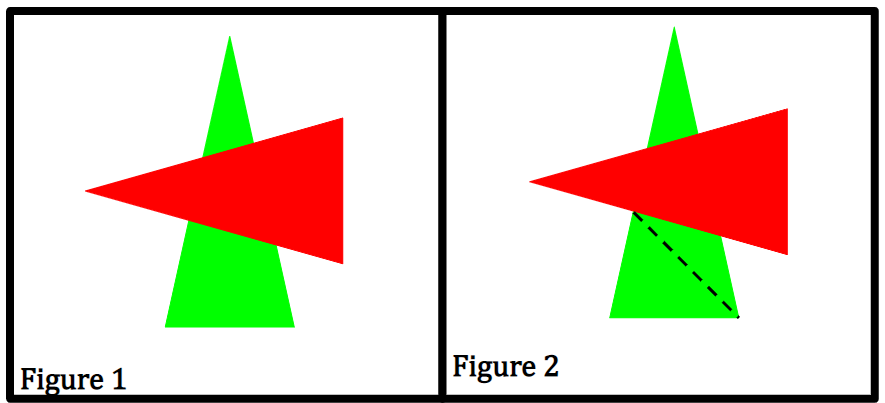
\includegraphics[scale=0.5]{../assets/hidden1.png}
    \end{center}
    With geometric analysis, the bottom part of the green triangle would be broken up into two triangles; in other words, the green triangle would be broken up into three pieces. 

    \bigskip 

    It's not hard to see that there are some significant disadvantages here. In particular: 
    \begin{itemize}
        \item You need to know \emph{all} of the triangles ahead of time. 
        \item You need a sophisticated algorithm. 
        \item You need to redo this process when the viewer moves. 
    \end{itemize}


    \item \underline{Painter's Algorithm:} The idea is that you \emph{sort} the triangles so that the furthest triangles from the camera/viewpoint get rendered first, and then you successively render the closer triangles, thus letting the closer triangles overwrite the farther triangles. The algorithm can roughly be written like so: 
    \begin{verbatim}
        Sort triangles in (reverse) order from viewpoint.
            Farthest triangles from view are first in list of triangles 
            Closest triangles from view are last in list of triangles 
        Render farther triangles first and closer ones last. 
            The closer ones overwrite the portions of the ones they hide.\end{verbatim}
    For example, suppose we have three triangles where the green triangle is the farthest from the viewer, the red triangle is the next farthest, and the blue triangle is the closest. 
    \begin{center}
        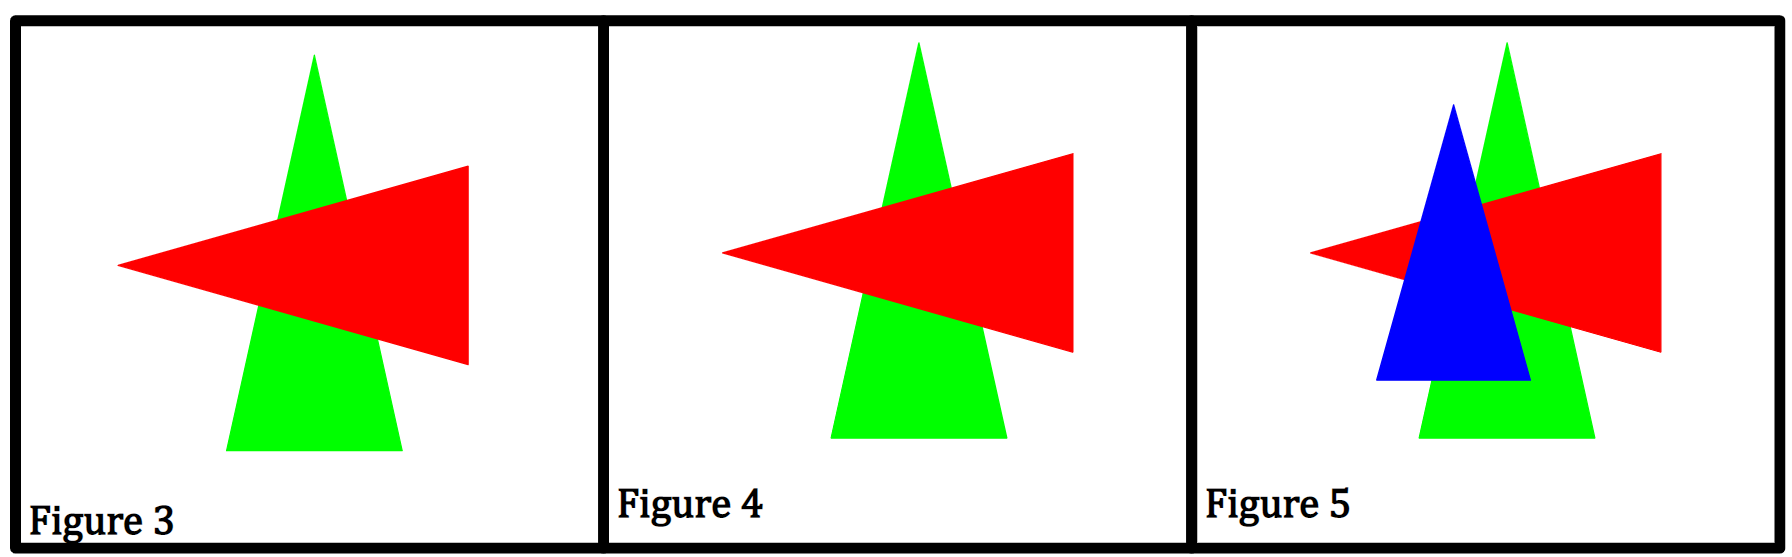
\includegraphics[scale=0.4]{../assets/hidden2.png}
    \end{center}
    Figure 3 shows the green triangle being rendered first. Figure 4 shows the red triangle being rendered next, thus hiding portions of the green triangle's pixels. Figure 5 shows the blue triangle being rendered next, hiding portions of the green and red triangle's pixels. 

    \bigskip 

    One obvious advantage is that it's elegant. All you need to do is sort and render. However, like with Geometric Analysis, there are some disadvantages:
    \begin{itemize}
        \item You need to know \emph{all} of the triangles ahead of time so you can sort them. 
        \item You need to redo this process when the viewer moves. 
        \item It may not be possible to sort consistently by distance. In particular, suppose you have interleaved triangles, like seen in figure 6. 
        \begin{center}
            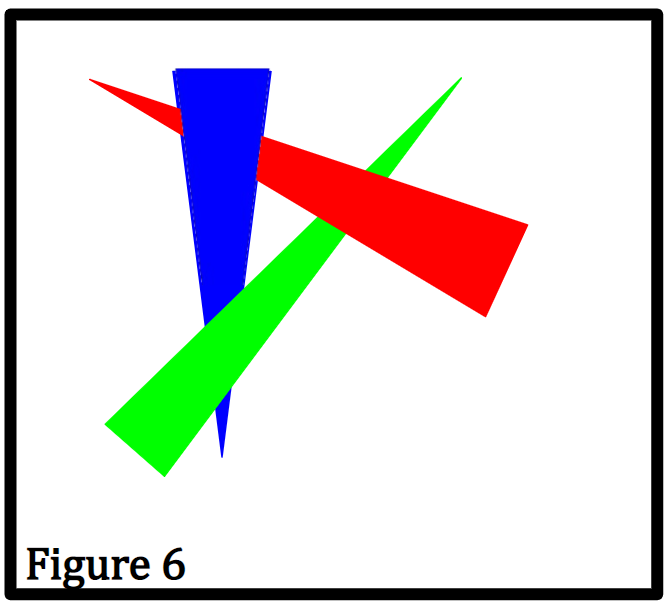
\includegraphics[scale=0.4]{../assets/hidden3.png}
        \end{center}
    \end{itemize}



    \item \underline{Depth Buffer:} This takes advantages of the fact that we're drawing into pixels. The idea is that you give each pixel two values; you give the pixel a color value \underline{and} a \textbf{depth} value, or (essentially) the distance from the viewer. A rough algorithm is as follows: 
    \begin{verbatim}
        Render triangles to pixels in any order. For each triangle: 
            Compare its depth to the previously written depth. 
            Keep the closer pixel color/depth values. 
    \end{verbatim}

    The advantages are: 
    \begin{itemize}
        \item It's simple. 
        \item You can render triangles in any order (so no need to sort).
        \item This can be done in parallel. Amenable to parallel computing.
    \end{itemize}

    The disadvantages are: 
    \begin{itemize}
        \item You need extra memory for the depth values\footnote{Memory is cheap, so this isn't too bad.}. 
        \item Aliasing problems.  
    \end{itemize}
\end{enumerate}


\subsection{Animations}
To give the appearance of motion, we show a succession of still images changing very rapidly.

\bigskip 

In OpenGL, we maintain two frame buffers\footnote{A buffer where we write an image.}:
\begin{itemize}
    \item \underline{Front buffer:} The current image being displayed. 
    \item \underline{Back buffer:} The next image to be displayed.  
\end{itemize} 
So, while the user is watching the front buffer, the back buffer is being processed (the next image that is being created). Then, you can just swap the buffers to switch the back buffer and the front buffers. 


\end{document}